\documentclass[convert={density=300,size=1080x800,outext=.png}]{standalone}

\usepackage{tikz}
\usetikzlibrary{decorations.pathreplacing}
\usetikzlibrary{arrows,positioning}
\tikzset{
    %Define standard arrow tip
    >=stealth',
    %Define style for boxes
    punkt/.style={
           rectangle,
           rounded corners,
           draw=black, very thick,
           text width=6.5em,
           minimum height=2em,
           text centered},
    % Define arrow style
    pil/.style={
           ->,
           thick}
}


\begin{document}

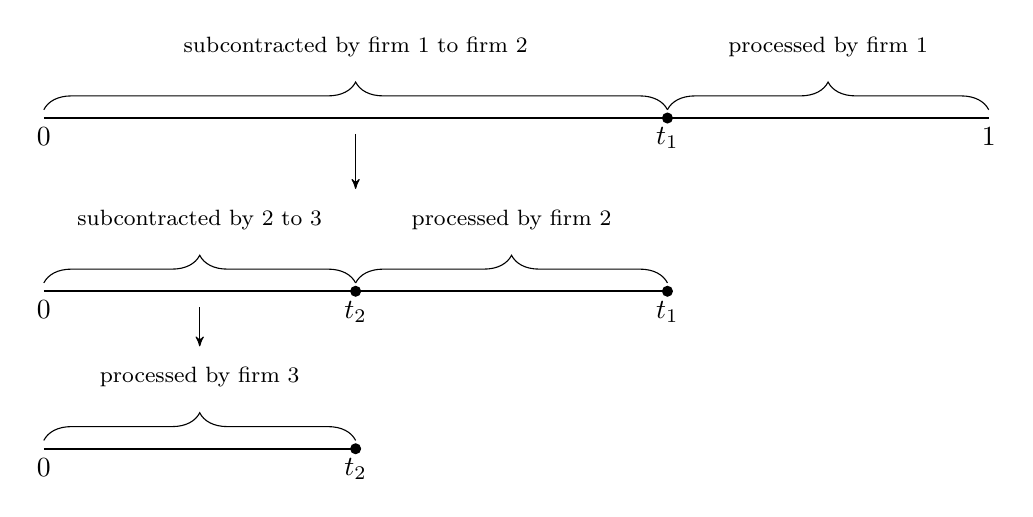
\begin{tikzpicture}[scale=1]

  \def\linelen{12}
  \def\tone{0.66 * \linelen};
  \def\ttwo{0.33 * \linelen};
  \def\levtwo{-2.2}; % level 2
  \def\levthree{-4.2}; % level 2

  \draw[thick] (0,0) -- (\linelen,0);

  \node at (0,0) [below] {$0$};
  \node at (\linelen,0) [below] {$1$};
  \fill (\tone,0) circle (2pt) node [below] {$t_1$};

  \draw [decorate,decoration={brace,amplitude=10pt},xshift=0pt,yshift=3pt]
    (\tone,0) -- (\linelen,0) node [black,midway,yshift=0.8cm] {\footnotesize
    processed by firm 1};
  \draw [decorate,decoration={brace,amplitude=10pt},xshift=0pt,yshift=3pt]
    (0,0) -- (\tone,0) node [black,midway,yshift=0.8cm] {\footnotesize
    subcontracted by firm 1 to firm 2};

  \draw[->] (0.5 * \tone, -0.2) -- (0.5 * \tone, -0.9);

  \draw[thick] (0, \levtwo) -- (\tone, \levtwo);
  \node at (0,\levtwo) [below] {$0$};
  \fill (\tone,\levtwo) circle (2pt) node [below] {$t_1$};
  \fill (\ttwo,\levtwo) circle (2pt) node [below] {$t_2$};

  \draw [decorate,decoration={brace,amplitude=10pt},xshift=0pt,yshift=3pt]
(0,\levtwo) -- (\ttwo,\levtwo) node [black,midway,yshift=0.8cm] {\footnotesize
subcontracted by 2 to 3};
  \draw [decorate,decoration={brace,amplitude=10pt},xshift=0pt,yshift=3pt]
(\ttwo,\levtwo) -- (\tone,\levtwo) node [black,midway,yshift=0.8cm] {\footnotesize
processed by firm 2};

  \draw[->] (0.5 * \ttwo, -2.4) -- (0.5 * \ttwo, -2.9);

  \draw[thick] (0, \levthree) -- (\ttwo, \levthree);
  \node at (0,\levthree) [below] {$0$};
  \fill (\ttwo,\levthree) circle (2pt) node [below] {$t_2$};

  \draw [decorate,decoration={brace,amplitude=10pt},xshift=0pt,yshift=3pt]
(0,\levthree) -- (\ttwo,\levthree) node [black,midway,yshift=0.8cm] {\footnotesize
processed by firm 3};

\end{tikzpicture}

\end{document}
